\section{所有最長路徑}
    以下內容節錄自Antti Laaksonen 的 Competitive Programmer’s Handbook
    \author{Antti Laaksonen}
    \subsection{概念}
    我們接下來的問題是計算樹中每個節點開始的最長路徑長度。
    這可以看作是樹直徑問題的一般化,因為其中最大的路徑長度等於樹的直徑。
    同樣,這個問題可以在$O(n)$的時間內解決。

    以一個例子來說明,考慮以下樹:

    \begin{figure}[h]
        \centering
        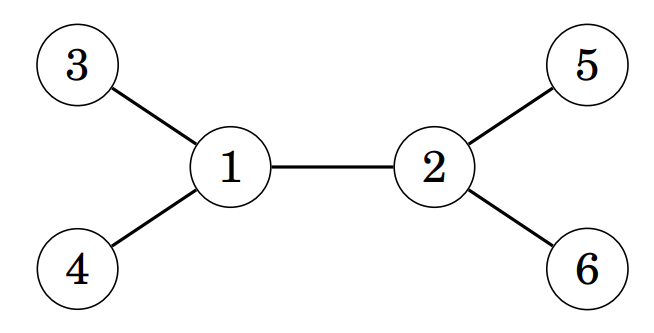
\includegraphics[width=0.5\textwidth]{../Images/Tree2.png}
    \end{figure}

    
    設 maxLength(x) 表示以節點 x 為起點的最長路徑長度。
    例如,在上面的樹中,maxLength(4) = 3,因為存在一條路徑 4 → 1 → 2 → 6。
    以下是完整的數值表:

    \begin{center}
    \begin{tabular}{|c|c|}
        \hline
        \text{Node} & \text{maxLength} \\
        \hline
        1 & 2 \\
        2 & 2 \\
        3 & 3 \\
        4 & 3 \\
        5 & 3 \\
        6 & 3 \\
        \hline
    \end{tabular}    
    \end{center}
    

    在解決這個問題時,一個好的起點是將樹任意地選擇一個節點作為根節點:

    \begin{figure}[h]
        \centering
        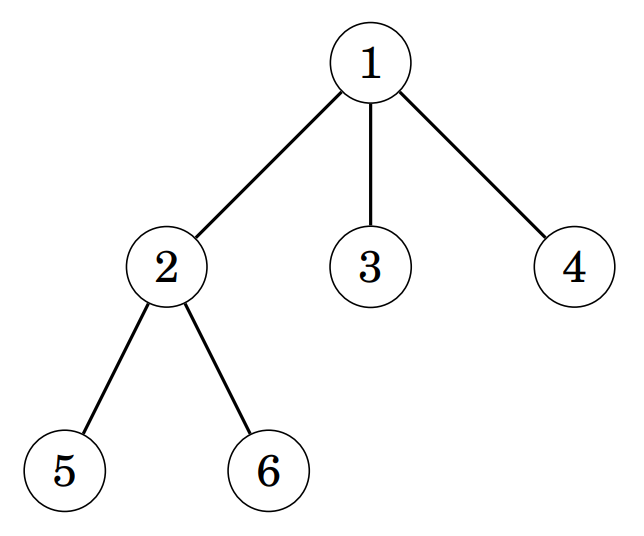
\includegraphics[width=0.5\textwidth]{../Images/Tree3.png}
    \end{figure}

    問題的第一部分是計算每個節點 x 通過其子節點的最大路徑長度。例如,從節點 1 出發的最長路徑通過其子節點 2。

    這部分可以在 $O(n)$ 的時間內輕鬆解決,因為我們可以使用動態規劃,就像之前所做的一樣。
    然後,問題的第二部分是計算每個節點 x 通過其父節點 p 的最大路徑長度。例如,從節點 3 出發的最長路徑通過其父節點 1。

    乍一看,似乎我們應該選擇從 p 開始的最長路徑。
    然而,這並不總是有效的,因為從 p 開始的最長路徑可能會經過 x。是一個範例:$2 \to 1 \to 4$。

    然而,我們仍然可以在 $O(n)$ 的時間內解決第二部分問題,方法是為每個節點 x 存儲兩個最大長度:

    \begin{itemize}
        \item $maxLength_1(x)$:從節點 x 出發的最長路徑的長度。
        \item $maxLength_2(x)$:從節點 x 出發的另一條方向的最長路徑的長度。
    \end{itemize}
    
    例如,在上面的圖中,$maxLength_1(x) = 2$。
    
    它使用路徑 1 → 2 → 5,而 $maxLength_2(x) = 1$,使用路徑 1 → 3。

    最後,如果對應於 $maxLength_1(p)$ 的路徑經過 x,我們可以得出最大長度為 $maxLength_2(p) + 1$;否則,最大長度為 $maxLength_1(p) + 1$。

    \subsection{小結}
    老實說我沒有在競賽中看過這樣的題目,不過這幾年我沒有看過的題目非常多,我認為也許會用到所以就翻譯這篇文章給你們閱讀。

    \subsection{範例與練習}

    \problem CSES task 1132 Tree Distances I 

    \textbf{題目敘述}

    給定一個由 n 個節點組成的樹。
    
    你的任務是找出每個節點到另一個節點的最大距離。

    \textbf{輸入說明}

    第一行輸入一個整數 $n$:節點的數量。這些節點被編號為 $1, 2,\cdots , n$。

    接下來有 $n-1$ 行描述邊。每行包含兩個整數 $a$ 和 $b$:表示節點 $a$ 和節點 $b$ 之間有一條邊。
    
    \textbf{輸出說明}

    輸出 $n$ 個整數:對於每個節點 $1, 2,\cdots , n$,輸出其到其他節點的最大距離。

    \textbf{範例測試}

    \begin{tabular}{|m{7cm}|m{7cm}|}
        \hline
        範例輸入 1 & 範例輸出 1 \\
        \hline
        \verb|5|  & \verb|2 3 2 3 3| \\
        \verb|1 2| & \\
        \verb|1 3|  & \\
        \verb|3 4|  & \\
        \verb|3 5|  & \\
        \hline
    \end{tabular}